\section{DrawAFriend: The Game}

\begin{figure}
  \centering%
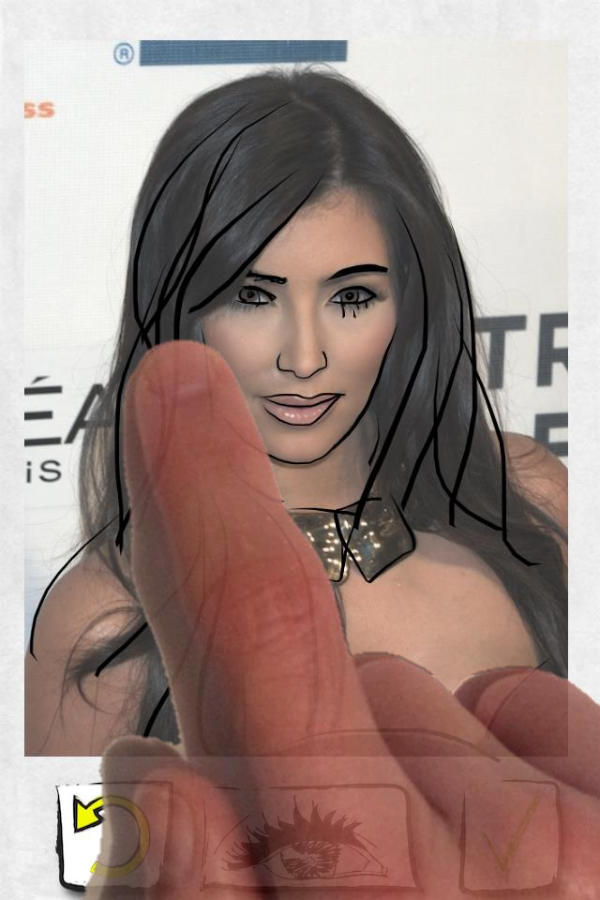
\includegraphics[width=1.5in]{DaF/kim_finger.pdf}
\hspace{0.1in}
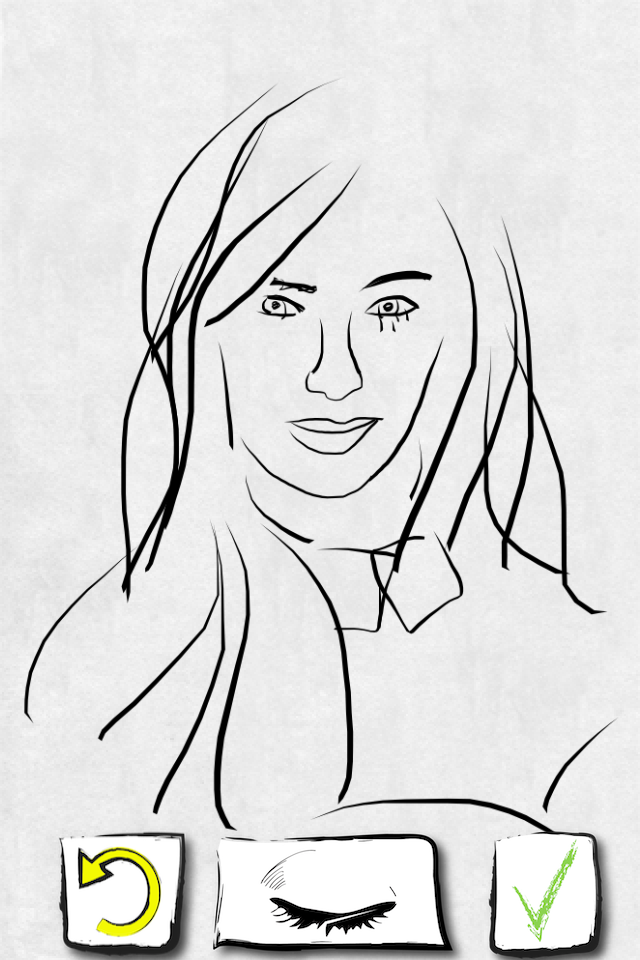
\includegraphics[width=1.5in]{DaF/kim_hidden.png}
  \caption{DrawAFriend: tracing a photo (left), the drawing alone (right).}
  \label{fig:DaF}
\end{figure}

\begin{figure}
  \centering%
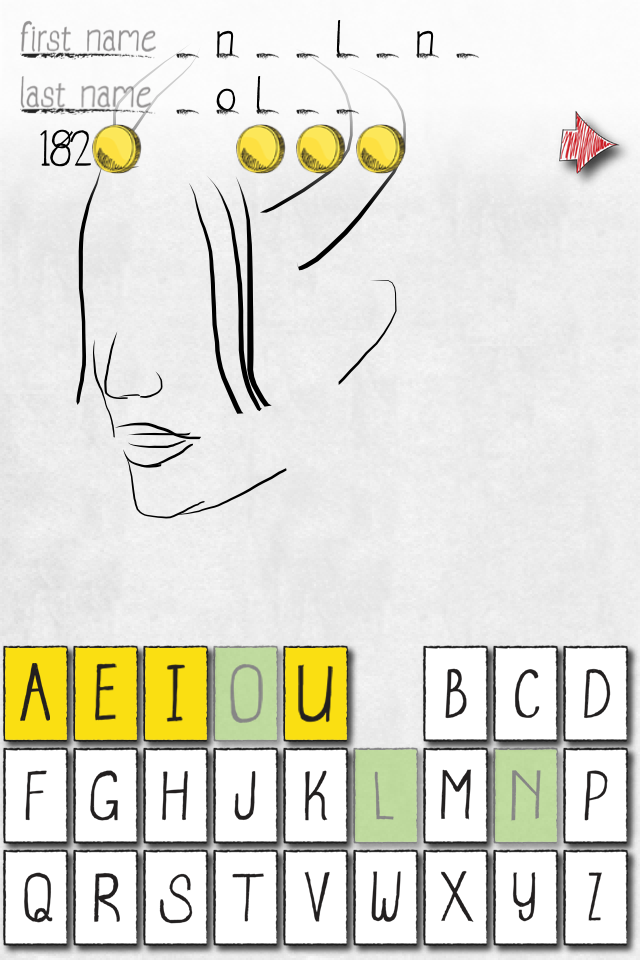
\includegraphics[width=1.5in]{DaF/angelina_guess1.png}
\hspace{0.1in}
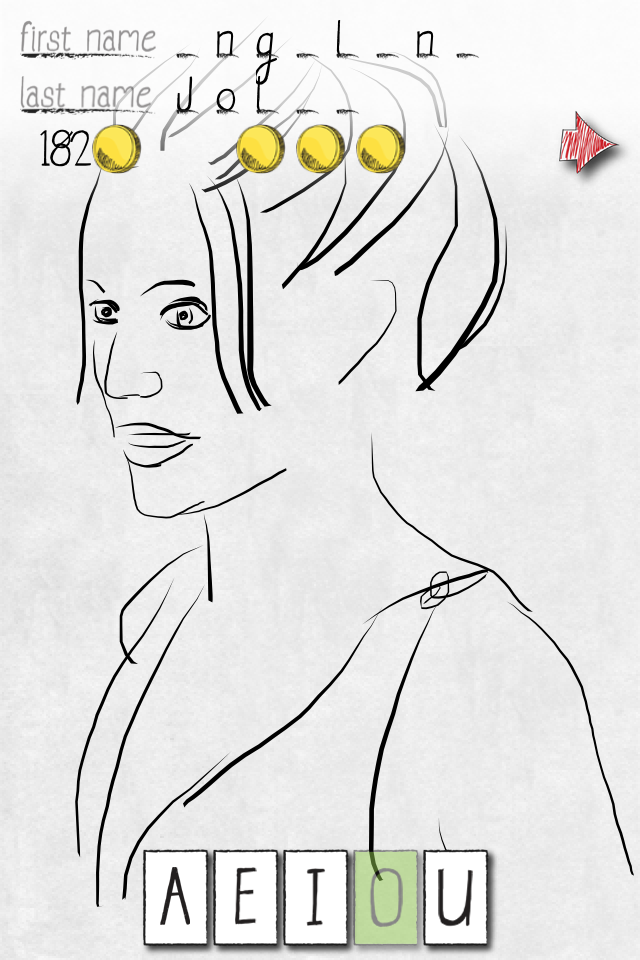
\includegraphics[width=1.5in]{DaF/angelina_guess2.png}
  \caption{DrawAFriend: guessing identity (left). Once a player guesses all consonants in a name, the consonant keys animate away and vowels no longer cost coins. (right).}
  \label{fig:DaF2}
\end{figure}

We have developed \daf, a Facebook-integrated turn-based drawing and guessing game for mobile devices.  It works as follows. Players have an option to start a game with either a Facebook friend or a random other player.  The player is then given four pictures which he can draw. These will either be mutual Facebook friends' profile pictures or  celebrity photos. In the case of a random player, only celebrity photos are offered to draw.

After choosing a photo to draw, the player is brought to the drawing screen. There she can trace the image (see Figure~\ref{fig:DaF} left). At any point, the user can press the {\em eye} button to hide the photo and see their drawing on its own (Figure~\ref{fig:DaF} right). To overcome the limitations of the phone's size, and touch screen inaccuracies, players can pan and zoom using the pinch zoom, and two fingered pan gestures.

Once finished, the player sends her drawing to the friend or random player with whom she is playing. The friend receives a notification that they have a drawing to guess. Once the drawing is complete, the user is prompted to guess the identity of the other player's drawing (Figure~\ref{fig:DaF2} left). The drawing is replayed, and similar to {\em Hangman}, the player can guess which letters are in the mutual friend or celebrity's name. Vowels originally cost coins, however once all the consonants are guessed the final vowels are offered for free to complete the guess (Figure~\ref{fig:DaF2} right).

This tracing paradigm results in a set of pre-aligned drawings. Whereas other papers begin with rasterized versions of drawings, we collect individual strokes represented as polylines along with timing information.  Furthermore, by observing the guesses we can indirectly evaluate the quality of the drawings. We hypothesize that a good drawing is much more likely to be guessed correctly than a bad drawing. DrawAFriend thus leverages a dataset of quality photos (Faceboook profile pictures and celebrity images) and via the efforts of players, results in a large dataset of user created drawings. This dataset includes drawings from artists around the world with different artistic and cultural backgrounds.

For the purposes of tackling the fat finger problem, we focus for the remainder of the paper on the corpus of celebrity drawings. These represent sets of drawings of the same photographs by many different artists.